\documentclass[conference]{IEEEtran}
\IEEEoverridecommandlockouts
\usepackage{cite}
\usepackage{amsmath,amssymb,amsfonts}
\usepackage{graphicx}
\usepackage{textcomp}
\usepackage{xcolor}
\usepackage{array}
\usepackage{tikz}
\usetikzlibrary{positioning,arrows.meta}
\newcolumntype{L}[1]{>{\raggedright\arraybackslash}p{#1}}
\graphicspath{{figures/}}
\hyphenation{Edge-IIoTset BiLSTM}
\usepackage[hidelinks]{hyperref}% clickable [n] citations and cross-references, no colored boxes
\renewcommand{\arraystretch}{1.0}% table row spacing; 1.05 or more pushes the paper to 7 pages
% Starts a new, centered row of author blocks. IEEEtran only centers the author
% list as a whole, so a row it wraps by itself drifts sideways. Use \linebreakand
% after every third author and \and between authors on the same row.
\makeatletter
\newcommand{\linebreakand}{\end{@IEEEauthorhalign}\hfill\mbox{}\par
  \mbox{}\hfill\begin{@IEEEauthorhalign}}
\makeatother
\begin{document}

\title{Same-Dataset Accuracy Does Not Transfer: Cross-Dataset Evaluation of Intrusion Detectors on WSN-DS, CICIoT2023, and Edge-IIoTset}

% One block per author, three per row. A 5th or 6th author goes after Shaik Gafar
% with \and; a 7th starts a third row with \linebreakand.
% TODO: Mogili Vikas Goud's and Shaik Gafar's emails go on the last line of their blocks.
\author{\IEEEauthorblockN{Riteesh Thiruveedhula}
\IEEEauthorblockA{\textit{Dept. of CSE-AIML} \\
\textit{K G Reddy College of Engineering}\\
\textit{and Technology}, Hyderabad, India \\
riteesh.vnsp@gmail.com}
\and
\IEEEauthorblockN{Velagala Sai Tarun Reddy}
\IEEEauthorblockA{\textit{Dept. of CSE-AIML} \\
\textit{K G Reddy College of Engineering}\\
\textit{and Technology}, Hyderabad, India \\
saitarunrdy@gmail.com}
\and
\IEEEauthorblockN{Mogili Vikas Goud}
\IEEEauthorblockA{\textit{Dept. of CSE-AIML} \\
\textit{K G Reddy College of Engineering}\\
\textit{and Technology}, Hyderabad, India}
\linebreakand
\IEEEauthorblockN{Shaik Gafar}
\IEEEauthorblockA{\textit{Dept. of CSE-AIML} \\
\textit{K G Reddy College of Engineering}\\
\textit{and Technology}, Hyderabad, India}
}

\maketitle

\begin{abstract}
Intrusion detection models are usually trained and tested on a single benchmark, which says little about how they behave on traffic from another network. We measure this on three public wireless and Internet of Things security datasets, WSN-DS, CICIoT2023, and Edge-IIoTset, after mapping their attack labels to a shared five-class taxonomy. The models are Random Forest and XGBoost baselines, a hybrid convolutional-recurrent model with self-attention, and a domain adversarial neural network that reuses the hybrid encoder and is trained on pooled data from two of the datasets. Each model is scored on held-out test data from the datasets it was trained on. Random Forest and the hybrid model are also trained on each dataset and tested on the other two. Same-dataset accuracy ranges from 91.9\% to 99.6\%. Cross-dataset accuracy is at most 67.6\% for Random Forest and 80.7\% for the hybrid model, and every Random Forest transfer score falls below the share of the largest class in the target test set. On Edge-IIoTset, Random Forest reaches 92.1\% accuracy but only 65.9\% macro-F1. The adversarial model scores 1.1 to 1.3 points below the hybrid model trained on each dataset separately. Scoring protocols differ between models, and we list each difference. For these datasets, same-dataset accuracy alone is not sufficient evidence, and a transfer claim needs matched scoring protocols, per-class metrics, and repeated runs.
\end{abstract}

\begin{IEEEkeywords}
cross-dataset evaluation, domain adaptation, Internet of Things, intrusion detection, wireless sensor networks
\end{IEEEkeywords}

\section{Introduction}
Wireless sensor networks and Internet of Things (IoT) deployments expose many resource-constrained devices to denial-of-service, spoofing, and reconnaissance attacks. Studies of learning-based intrusion detection systems (IDSs) report very high accuracy on individual benchmarks. Such a score measures how well a model recognizes attacks produced by the capture process, feature extractor, and label set it was trained on. A deployed detector sees a different network and a different measurement pipeline. Sommer and Paxson argued that machine learning for intrusion detection calls for especially careful evaluation \cite{sommer2010}.

We measure the gap between same-dataset and cross-dataset results on three public benchmarks that differ in network layer and measurement level: WSN-DS \cite{almomani2016}, CICIoT2023 \cite{neto2023}, and Edge-IIoTset \cite{ferrag2022}. We ask (i) how same-dataset results compare with results when a model trained on one dataset is tested on another; (ii) whether tree ensembles and a hybrid network behave differently under the two evaluations, where the hybrid combines a convolutional neural network (CNN), a bidirectional long short-term memory (BiLSTM) network, and attention; and (iii) whether a domain adversarial neural network (DANN) \cite{ganin2016} trained on two pooled datasets changes same-dataset results relative to per-dataset training. Our contributions are:
\begin{itemize}
\item a shared five-class label mapping and two feature tracks for the three datasets, documented in Tables~\ref{tab:labels} and~\ref{tab:slots};
\item same-dataset results for Random Forest (RF) \cite{breiman2001}, XGBoost \cite{chen2016}, the hybrid model, and DANN, plus confusion-matrix metrics for the two tree baselines, which show that RF's 92.1\% accuracy on Edge-IIoTset comes with a macro-F1 of 65.9\%;
\item transfer matrices for RF and the hybrid model, in which every RF transfer accuracy is below the share of the largest class in the target test set;
\item a list of the protocol differences between experiments (Table~\ref{tab:protocol}), which limit what the comparisons can show.
\end{itemize}

\section{Related Work}\label{sec:related}
WSN-DS covers four denial-of-service attacks on wireless sensor networks running the low-energy adaptive clustering hierarchy (LEACH) protocol \cite{heinzelman2000,almomani2016}. CICIoT2023 contains 33 attacks in seven categories executed against 105 IoT devices \cite{neto2023}. Edge-IIoTset was generated on an IoT and industrial IoT (IIoT) testbed and contains 14 attacks in five categories \cite{ferrag2022}.

Surveys of deep learning for intrusion detection catalog architectures, datasets, and comparisons \cite{ferrag2020}. RF \cite{breiman2001} and gradient-boosted trees in XGBoost \cite{chen2016} are standard strong baselines on tabular network features. Hybrid networks combining convolutions, long short-term memory (LSTM) \cite{hochreiter1997} in bidirectional form \cite{schuster1997}, and attention \cite{vaswani2017} are common in recent IDS work, for example on wireless IoT sensor networks \cite{phalaagae2025}. Our hybrid model belongs to this family; we configured it ourselves and did not reproduce that work.

Cross-dataset studies of network intrusion detection report large drops when a model is tested on a dataset it was not trained on \cite{dhooge2023,layeghy2022}, including macro-F1 losses of up to 30 points for federated models moved between Edge-IIoTset, CICIoT2023, and TII-SSRC-23 \cite{bilal2026}. We add a wireless sensor network dataset and compare each RF transfer score with the target's majority-class share.

Each network intrusion detection dataset ships with its own feature set, which makes models hard to compare across datasets. Sarhan et al.\ address this by re-expressing datasets in a common NetFlow-based feature set \cite{sarhan2021}. Our behavioral track (Section~\ref{sec:features}) is a cruder approach that maps feature slots by hand, and it has not been validated as a common representation. Domain adaptation theory bounds target error by source error plus a domain divergence \cite{bendavid2010}, and Pan and Yang survey transfer learning \cite{pan2010}. DANN connects a domain classifier to a shared feature extractor through a gradient reversal layer, so training pushes the extractor toward domain-invariant features \cite{ganin2015,ganin2016}. Ganin et al.\ formulated it for labeled source data and unlabeled target data \cite{ganin2016}. Our DANN experiment uses labels from both domains (Section~\ref{sec:protocol}).

\section{Datasets and Label Mapping}\label{sec:data}
We obtained the three datasets as tabular copies from Kaggle. The WSN-DS and CICIoT2023 listings are not under the original authors' names, and we did not verify their contents against the original releases. The archived loader draws a class-stratified sample of about 200{,}000 records per dataset (at least 200 per class, the rest in proportion to class frequency). For CICIoT2023 and Edge-IIoTset, the saved baseline test sets (Table~\ref{tab:datasets}) fit this cap, but the WSN-DS test set shows that WSN-DS was used in full. We split each dataset 70/10/20 into training, validation, and test partitions, stratified by class, and the archived code uses seed 42 for sampling and splitting.

\begin{table}[t]
\caption{Baseline Test Sets (20\% Stratified Split)}
\label{tab:datasets}
\centering
\footnotesize
\setlength{\tabcolsep}{5pt}
\begin{tabular}{|l|l|c|c|}
\hline
\textbf{Dataset} & \textbf{Classes} & \textbf{Test size: class counts} & \textbf{Majority} \\
\hline
WSN-DS & 0,1,2,3 & 74{,}933: 68{,}014/1{,}328/4{,}929/662 & 90.8\% \\
\hline
CICIoT2023 & 0,2,3,4 & 39{,}997: 934/421/38{,}307/335 & 95.8\% \\
\hline
Edge-IIoTset & 0,2,3,4 & 39{,}999: 29{,}121/22/6{,}092/4{,}764 & 72.8\% \\
\hline
\multicolumn{4}{p{231pt}}{Counts follow the class order and come from the saved baseline confusion matrices. Majority: share of the largest class. The composition of the hybrid and DANN test sets was not saved.}
\end{tabular}
\end{table}

We map raw labels to a five-class project taxonomy (Table~\ref{tab:labels}) and discard records whose label is not in the mapping. We built the taxonomy by judgment and did not validate it. Class~1 (``Jamming'') holds only WSN-DS time-division multiple access (TDMA) scheduling attacks and does not occur in the other datasets. Class~2 (``Spoofing'') puts blackhole and grayhole routing misbehavior in WSN-DS together with ARP spoofing, DNS spoofing, and man-in-the-middle traffic in the other two. These are different mechanisms, and the datasets observe them through different features. Since the label sets differ, cross-dataset scoring must decide what to do with a class that only one side has (Section~\ref{sec:protocol}).

\begin{table*}[t]
\caption{Label Mapping From Dataset Attack Labels to the Five-Class Taxonomy}
\label{tab:labels}
\centering
\footnotesize
\setlength{\tabcolsep}{5pt}
\begin{tabular}{|L{2.3cm}|L{2.5cm}|L{6.1cm}|L{5.4cm}|}
\hline
\textbf{Class} & \textbf{WSN-DS} & \textbf{CICIoT2023} & \textbf{Edge-IIoTset} \\
\hline
0 Normal & Normal & BenignTraffic & Normal \\
\hline
1 Jamming$^{\mathrm{a}}$ & TDMA & -- & -- \\
\hline
2 Spoofing & Blackhole, Grayhole & MITM-ArpSpoofing, DNS\_Spoofing & MITM \\
\hline
3 DoS\_Flood & Flooding & 19 labels: DDoS-*, DoS-*, and Mirai flood variants (e.g., DDoS-SYN\_Flood, DoS-UDP\_Flood, Mirai-udpplain) & DDoS\_UDP, DDoS\_ICMP, DDoS\_TCP, DDoS\_HTTP \\
\hline
4 Intrusion\_Probe & -- & 12 labels: Recon-* (four), VulnerabilityScan, CommandInjection, SqlInjection, XSS, BrowserHijacking, Backdoor\_Malware, DictionaryBruteForce, Uploading\_Attack & SQL\_injection, Password, Vulnerability\_scanner, Uploading, Backdoor, Port\_Scanning, XSS, Ransomware, Fingerprinting \\
\hline
\multicolumn{4}{p{\dimexpr16.3cm+6\tabcolsep\relax}}{$^{\mathrm{a}}$The class keeps the name used in the project taxonomy although it contains only scheduling attacks. A dash means the dataset has no records mapped to that class.}
\end{tabular}
\end{table*}

\section{Methods}\label{sec:methods}
\subsection{Feature Tracks and Preprocessing}\label{sec:features}
The \emph{behavioral track} defines 20 named slots (volume, rate, send/receive ratio, acknowledgement ratio, and so on) and fills each one with a hand-written expression over each dataset's own columns. Only the slot names are shared. As Table~\ref{tab:slots} shows, the ``energy'' slot holds expended energy in WSN-DS, total packet size in CICIoT2023, and a UDP stream index in Edge-IIoTset. Same-dataset evaluation uses a \emph{native track}. For WSN-DS and CICIoT2023 it has the same 20 columns as the behavioral track. For Edge-IIoTset it has 35 raw protocol fields (e.g., TCP flags, sequence and acknowledgement values, and DNS, MQTT, and Modbus fields) that we chose for class discrimination.

\begin{table*}[t]
\caption{Examples of Behavioral Feature Slot Definitions per Dataset}
\label{tab:slots}
\centering
\footnotesize
\setlength{\tabcolsep}{5pt}
\begin{tabular}{|L{2.0cm}|L{5.0cm}|L{3.4cm}|L{5.4cm}|}
\hline
\textbf{Slot} & \textbf{WSN-DS} & \textbf{CICIoT2023} & \textbf{Edge-IIoTset} \\
\hline
volume & \texttt{DATA\_S}+\texttt{DATA\_R} & \texttt{Tot sum} & \texttt{tcp.len}+\texttt{mqtt.len} \\
\hline
ack ratio & \texttt{ADV\_R}/(\texttt{ADV\_S}+1) & \texttt{ack\_count}/\texttt{Number} & \texttt{tcp.flags.ack} \\
\hline
energy & \texttt{Expaned Energy} & \texttt{Tot size} & \texttt{udp.stream} \\
\hline
port entropy & \texttt{Rank}/(max \texttt{Rank}+1) & \texttt{Covariance} & $|$\texttt{tcp.srcport}$-$\texttt{tcp.dstport}$|$/(sum+1) \\
\hline
mqtt activity & constant 0 & \texttt{DNS}+\texttt{DHCP}+\texttt{ARP} & \texttt{mqtt.len}+\texttt{mqtt.ver} \\
\hline
\multicolumn{4}{p{\dimexpr15.8cm+6\tabcolsep\relax}}{Entries are the dataset column names used in the slot expressions; spellings follow the datasets.}
\end{tabular}
\end{table*}

Fig.~\ref{fig:pipeline} summarizes preprocessing. We pass each value through a signed logarithm,
\begin{equation}
\tilde{x} = \operatorname{sign}(x)\,\log\!\bigl(1+|x|\bigr),
\label{eq:log}
\end{equation}
and clip it to $[-50,50]$. Both steps act on single values, so applying them before the split leaks no information. After the stratified split, the RF and XGBoost runs apply the synthetic minority oversampling technique (SMOTE) \cite{chawla2002} to the training partition. We then fit a robust scaler on the training partition (after oversampling, for the baselines) and apply it to all partitions, separately for each dataset. For the deep models, we cut each partition into windows of $T=5$ consecutive rows and label each window by its last row. The split shuffles rows, so the rows in a window are usually not adjacent in the original capture.

\begin{figure}[t]
\centering
\scriptsize
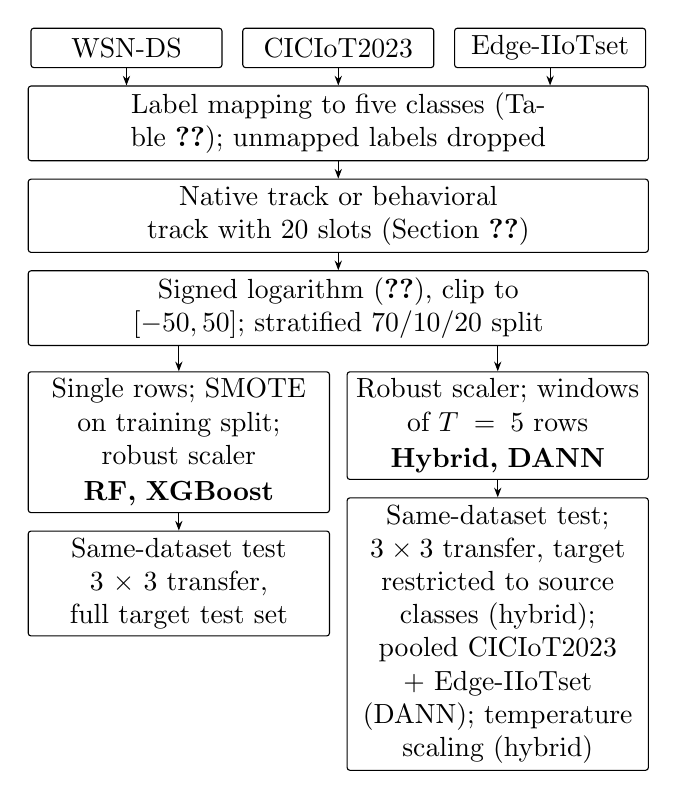
\begin{tikzpicture}[
  box/.style={draw, rounded corners=1pt, align=center, inner sep=2.5pt, minimum height=0.5cm},
  wide/.style={box, text width=7.7cm},
  half/.style={box, text width=3.65cm},
  arr/.style={-{Stealth[length=3.5pt]}},
  node distance=0.22cm]
\node[box, text width=2.25cm] (c) {CICIoT2023};
\node[box, text width=2.25cm, left=0.25cm of c] (w) {WSN-DS};
\node[box, text width=2.25cm, right=0.25cm of c] (e) {Edge-IIoTset};
\node[wide, below=of c] (lab) {Label mapping to five classes (Table~\ref{tab:labels}); unmapped labels dropped};
\node[wide, below=of lab] (feat) {Native track or behavioral track with 20 slots (Section~\ref{sec:features})};
\node[wide, below=of feat] (pre) {Signed logarithm \eqref{eq:log}, clip to $[-50,50]$; stratified 70/10/20 split};
\node[half, below=0.32cm of pre.south west, anchor=north west] (rows) {Single rows; SMOTE on training split; robust scaler\\[1pt] \textbf{RF, XGBoost}};
\node[half, below=0.32cm of pre.south east, anchor=north east] (win) {Robust scaler; windows of $T=5$ rows\\[1pt] \textbf{Hybrid, DANN}};
\node[half, below=of rows] (ev1) {Same-dataset test\\ $3\times3$ transfer, full target test set};
\node[half, below=of win] (ev2) {Same-dataset test; $3\times3$ transfer, target restricted to source classes (hybrid); pooled CICIoT2023 + Edge-IIoTset (DANN); temperature scaling (hybrid)};
\foreach \s in {w,c,e} \draw[arr] (\s.south) -- (\s.south |- lab.north);
\draw[arr] (lab) -- (feat);
\draw[arr] (feat) -- (pre);
\draw[arr] (rows.north |- pre.south) -- (rows.north);
\draw[arr] (win.north |- pre.south) -- (win.north);
\draw[arr] (rows) -- (ev1);
\draw[arr] (win) -- (ev2);
\end{tikzpicture}
\caption{Experimental pipeline. The baselines and deep models share the first three stages and differ after the split (Table~\ref{tab:protocol}). Each dataset is scaled with its own robust scaler.}
\label{fig:pipeline}
\end{figure}

\subsection{Models}\label{sec:models}
\subsubsection{Baselines} RF \cite{breiman2001} is a strong baseline for tabular data that needs little tuning. We use the scikit-learn implementation \cite{pedregosa2011} with 100 trees, a fixed random seed, and default settings otherwise. We include XGBoost \cite{chen2016} to see whether gradient boosting behaves differently from bagged trees. It uses 100 trees, maximum depth 6, learning rate 0.1, and a multiclass softmax-probability objective.

\subsubsection{Hybrid CNN-BiLSTM-attention} This model, our own configuration of the hybrid family in \cite{phalaagae2025}, tests whether a learned representation transfers differently from trees. Two one-dimensional convolutions (kernel 3, 32 then 64 channels, batch normalization, ReLU, dropout 0.2) feed a two-layer bidirectional LSTM with 128 units per direction and dropout 0.3 between layers. Next come a single-head self-attention layer \cite{vaswani2017}, $\operatorname{softmax}(QK^{\top}/\sqrt{256})\,V$ with $Q$, $K$, and $V$ learned linear projections of the 256-dimensional outputs, an average over the five time steps, and a head $256\to128\to C$ (ReLU, dropout 0.3), where $C$ is the number of classes in the training data. Training uses AdamW \cite{loshchilov2019} (learning rate $10^{-3}$, weight decay $10^{-4}$), batch size 256, and at most 20 epochs. The learning rate halves after three epochs without validation improvement, and early stopping has patience 7 on validation loss. The loss is cross-entropy with class weights $w_c=\min\{5,\max\{0.5,\,N/(C\,n_c)\}\}$, where $n_c$ is the number of training windows of class $c$ and $N$ the total.

\subsubsection{DANN} DANN \cite{ganin2016} trains features that do not reveal which domain a sample came from, a property a cross-dataset detector would want. It reuses the hybrid encoder, whose 256-dimensional output feeds a threat head and, through a gradient reversal layer, a domain head ($256\to128\to2$). The loss is $\mathcal{L}_{\mathrm{threat}}+\lambda\,\mathcal{L}_{\mathrm{domain}}$ with $\lambda=0.1$, a class-weighted threat loss, and an unweighted domain loss. The reversal strength is $\alpha(p)=2/(1+e^{-5p})-1$, where $p$ is the fraction of adversarial epochs completed, so $\alpha$ reaches about 0.98 in the last one. Training runs eight threat-only epochs and then up to 25 adversarial epochs. It uses the hybrid's optimizer and schedule, with early stopping at patience 7 on the combined validation loss.

\begin{table*}[t]
\caption{Protocol Differences Between Experiments}
\label{tab:protocol}
\centering
\footnotesize
\setlength{\tabcolsep}{5pt}
\begin{tabular}{|L{2.2cm}|L{3.6cm}|L{3.4cm}|L{3.4cm}|L{3.4cm}|}
\hline
\textbf{Aspect} & \textbf{RF / XGBoost} & \textbf{Hybrid, same-dataset} & \textbf{Hybrid, transfer} & \textbf{DANN (CIC + Edge)} \\
\hline
Feature track & 20-slot schema$^{\mathrm{a}}$ & Native (20; 35 for Edge-IIoTset) & Behavioral (20 slots) & Behavioral (20 slots) \\
\hline
Edge-IIoTset file & Not recorded$^{\mathrm{a}}$ & ``ML'' selected file & ``DNN'' selected file & ``DNN'' selected file \\
\hline
Input; balancing & One row; SMOTE & 5-row window; class weights & 5-row window; class weights & 5-row window; class weights \\
\hline
Transfer scoring & Full target test set & Not applicable & Target restricted to source classes & Not a transfer test \\
\hline
Saved metrics & Accuracy, weighted P/R/F1, FAR, confusion matrix & Accuracy, weighted F1 & Accuracy & Accuracy, weighted F1 \\
\hline
Training & 100 trees (XGBoost: depth 6, rate 0.1) & $\le$20 epochs & $\le$20 epochs & 8 + $\le$25 epochs, $\lambda=0.1$ \\
\hline
\multicolumn{5}{p{\dimexpr16cm+8\tabcolsep\relax}}{$^{\mathrm{a}}$The saved baseline results record neither the feature schema nor the input file. The archived baseline script applies the 20-slot schema to every dataset but is not consistent with the archived Edge-IIoTset loader, so the schema and file behind the saved Edge-IIoTset baseline numbers cannot be confirmed.}
\end{tabular}
\end{table*}

\subsection{Evaluation Protocols}\label{sec:protocol}
\emph{Same-dataset:} we train each model on a dataset's training partition and score it on that dataset's held-out test partition. \emph{Cross-dataset transfer:} a model trained on a source dataset is scored on the test partition of a target dataset, for all nine pairs, and the target test set is scaled with the target's own scaler. RF is scored on the full target test set, so target samples from classes the source never saw count as errors. For the hybrid model, the target test set is first restricted to classes present in the source dataset. The two protocols differ, so their accuracies should not be differenced directly. \emph{DANN:} we train it on the pooled training partitions of CICIoT2023 and Edge-IIoTset (each scaled with its own scaler) with threat labels from both domains, and score it on each dataset's own test partition. This is not a held-out-domain transfer test, and unlike the original formulation \cite{ganin2016}, the target domain is labeled.

\emph{Metrics:} we saved accuracy for every model. For RF and XGBoost we also saved weighted precision, recall, and F1, the false alarm rate (FAR, the fraction of Normal samples predicted as any attack class), and confusion matrices, from which we derive macro-F1 and balanced accuracy (mean per-class recall). For the hybrid model and DANN we saved accuracy and weighted F1, and for the transfer matrices only accuracy. To calibrate, we fit one temperature on the validation partition by minimizing negative log-likelihood \cite{guo2017} and compute expected calibration error (ECE) over 15 bins on the test partition. We ran each configuration once, and the saved deep-learning results do not record the model-initialization seed. Table~\ref{tab:protocol} summarizes the differences.

\section{Experimental Results}\label{sec:results}
\subsection{Same-Dataset Results}
RF and XGBoost lead the native-track hybrid model on WSN-DS and CICIoT2023 by 1.5 to 1.6 points (Table~\ref{tab:same}). On Edge-IIoTset the native-track hybrid leads with 94.39\%, against 92.06\% for RF and 91.92\% for XGBoost. Weighted F1 follows the same order wherever it was saved. DANN, trained on pooled CICIoT2023 and Edge-IIoTset data, scores 1.29 and 1.13 points below the per-dataset behavioral hybrid models, which use the same feature track and data files. We also tried a three-domain DANN that added WSN-DS. Project notes say it did not converge to a useful solution. We saved no metrics from that run and make no quantitative claim about it.

\begin{table*}[t]
\caption{Same-Dataset Test Accuracy and Weighted F1 (\%), Single Run}
\label{tab:same}
\centering
\footnotesize
\setlength{\tabcolsep}{5pt}
\begin{tabular}{|l|c|c|c|c|c|c|c|c|c|}
\hline
 & \multicolumn{5}{c|}{\textbf{Accuracy}} & \multicolumn{4}{c|}{\textbf{Weighted F1}} \\
\cline{2-10}
\textbf{Dataset} & \textbf{\textit{RF}} & \textbf{\textit{XGB}} & \textbf{\textit{Hybrid (native)}} & \textbf{\textit{Hybrid (behav.)}} & \textbf{\textit{DANN}} & \textbf{\textit{RF}} & \textbf{\textit{XGB}} & \textbf{\textit{Hybrid (native)}} & \textbf{\textit{DANN}} \\
\hline
WSN-DS & 99.60 & 99.56 & 98.06 & 97.79 & -- & 99.60 & 99.57 & 98.15 & -- \\
\hline
CICIoT2023 & 99.42 & 99.44 & 97.80 & 97.79 & 96.50 & 99.42 & 99.44 & 97.59 & 96.03 \\
\hline
Edge-IIoTset & 92.06 & 91.92 & 94.39 & 97.42 & 96.29 & 94.25 & 94.01 & 94.65 & 96.32 \\
\hline
\multicolumn{10}{p{404pt}}{XGB: XGBoost. ``Hybrid (native)'' and ``Hybrid (behav.)'' use the native and behavioral tracks; weighted F1 for the latter was not saved. A dash means the model was not trained on that dataset. Feature schemas and data files differ across columns (Table~\ref{tab:protocol}).}
\end{tabular}
\end{table*}

\begin{table*}[t]
\caption{Cross-Dataset Transfer Accuracy (\%): Rows Are Training Datasets, Columns Are Test Datasets}
\label{tab:transfer}
\centering
\footnotesize
\setlength{\tabcolsep}{5pt}
\begin{minipage}[t]{0.47\textwidth}
\centering
\textbf{(a) Random Forest, full target test set}\\[2pt]
\begin{tabular}{|l|c|c|c|}
\hline
 & \textbf{WSN-DS} & \textbf{CICIoT2023} & \textbf{Edge-IIoTset} \\
\hline
WSN-DS & \textbf{99.60} & 0.18 & 11.94 \\
\hline
CICIoT2023 & 1.26 & \textbf{99.42} & 26.30 \\
\hline
Edge-IIoTset & 1.90 & 67.64 & \textbf{92.06} \\
\hline
Majority share & 90.8 & 95.8 & 72.8 \\
\hline
\end{tabular}
\end{minipage}\hfill
\begin{minipage}[t]{0.47\textwidth}
\centering
\textbf{(b) Hybrid, target restricted to source classes}\\[2pt]
\begin{tabular}{|l|c|c|c|}
\hline
 & \textbf{WSN-DS} & \textbf{CICIoT2023} & \textbf{Edge-IIoTset} \\
\hline
WSN-DS & \textbf{97.79} & 0.30 & 80.70 \\
\hline
CICIoT2023 & 0.99 & \textbf{97.79} & 15.40 \\
\hline
Edge-IIoTset & 26.96 & 61.77 & \textbf{97.42} \\
\hline
Majority share & \multicolumn{3}{c|}{not saved} \\
\hline
\end{tabular}
\end{minipage}

\vspace{3pt}
\parbox{0.96\textwidth}{\footnotesize Bold entries are same-dataset results. ``Majority share'' is the largest class's share of the column dataset's RF baseline test set (Table~\ref{tab:datasets}). The panels differ in class handling, feature tracks, and training (Table~\ref{tab:protocol}) and are not directly comparable.}
\end{table*}

\subsection{Metrics Derived From Confusion Matrices}
Only RF and XGBoost have saved confusion matrices (Table~\ref{tab:cm}). Both reach macro-F1 near 97\% on WSN-DS, with FAR below 0.4\%. On CICIoT2023 their accuracy is 99.4\%, yet macro-F1 is only 88.3\% (RF) and 88.9\% (XGBoost), and FAR is 8.24\% and 9.31\%. Edge-IIoTset has the widest gap, with accuracy above 91.9\% and macro-F1 of 65.9\% and 65.5\%. On Edge-IIoTset, RF detects all 22 test samples of class~2 but also assigns 2{,}298 of the 6{,}092 class~3 samples (37.7\%) to class~2, so class~2 has a precision of 0.9\% (Fig.~\ref{fig:cm}). RF's recall on CICIoT2023 is near 100\% for class~3, which makes up 95.8\% of the test set, and 91.8\%, 79.3\%, and 82.1\% for the smaller classes.

\begin{table}[t]
\caption{Confusion-Matrix-Derived Metrics for the Baselines (\%)}
\label{tab:cm}
\centering
\footnotesize
\setlength{\tabcolsep}{4pt}
\begin{tabular}{|l|l|c|c|c|c|c|}
\hline
\textbf{Model} & \textbf{Dataset} & \textbf{Acc.} & \textbf{W-F1} & \textbf{Macro-F1}$^{\mathrm{a}}$ & \textbf{Bal. acc.}$^{\mathrm{a}}$ & \textbf{FAR} \\
\hline
RF & WSN-DS & 99.60 & 99.60 & 97.02 & 98.02 & 0.29 \\
\hline
RF & CICIoT2023 & 99.42 & 99.42 & 88.26 & 88.29 & 8.24 \\
\hline
RF & Edge-IIoTset & 92.06 & 94.25 & 65.93 & 87.10 & 0.59 \\
\hline
XGB & WSN-DS & 99.56 & 99.57 & 97.09 & 98.06 & 0.33 \\
\hline
XGB & CICIoT2023 & 99.44 & 99.44 & 88.86 & 89.42 & 9.31 \\
\hline
XGB & Edge-IIoTset & 91.92 & 94.01 & 65.51 & 86.93 & 0.58 \\
\hline
\multicolumn{7}{p{237pt}}{$^{\mathrm{a}}$Derived from the saved confusion matrices. W-F1: weighted F1; XGB: XGBoost.}
\end{tabular}
\end{table}

\begin{figure*}[t]
\centering
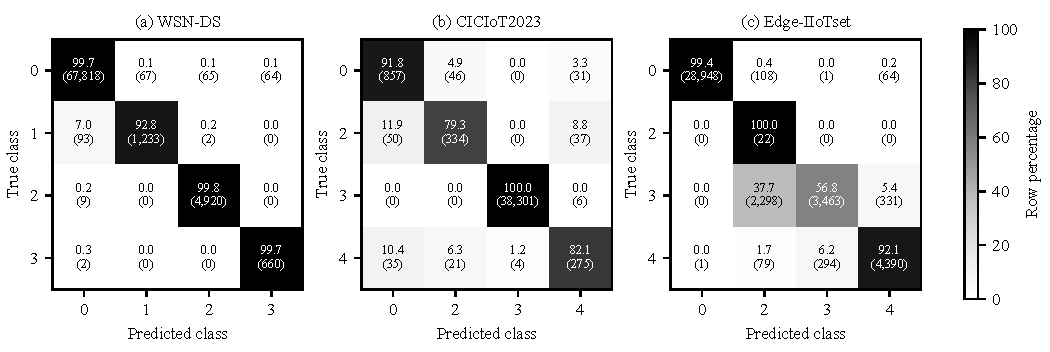
\includegraphics[width=0.92\textwidth]{fig_rf_cm.pdf}
\caption{Row-normalized confusion matrices of the Random Forest baseline on the held-out test sets: row percentage with the sample count in parentheses. Class identifiers follow Table~\ref{tab:labels}.}
\label{fig:cm}
\end{figure*}

\subsection{Cross-Dataset Transfer}
Off the diagonal of the transfer matrices (Table~\ref{tab:transfer}), RF accuracy ranges from 0.18\% to 67.64\% and hybrid accuracy from 0.30\% to 80.70\%. Between WSN-DS and CICIoT2023 both models score below 2\% in either direction. From Edge-IIoTset to WSN-DS the hybrid model reaches 26.96\%, against 1.90\% for RF. Every off-diagonal RF accuracy is below the majority-class share of its target test set. The hybrid scores use masked targets: a model trained on WSN-DS is tested only on classes 0, 2, and 3, tests on WSN-DS leave out class~1, and pairs between CICIoT2023 and Edge-IIoTset need no mask. We did not save the composition of the masked test sets.

\subsection{Calibration}
The fitted temperatures for the native-track hybrid models are 1.040 (WSN-DS), 1.495 (CICIoT2023), and 1.077 (Edge-IIoTset). Temperature scaling raised ECE on all three datasets, in the same order: from 1.70\% to 1.86\%, from 0.23\% to 0.43\%, and from 1.78\% to 2.04\%.

\section{Discussion and Limitations}\label{sec:discussion}
\subsection{Same-Dataset Versus Cross-Dataset Accuracy}
Every same-dataset result exceeds 91\% accuracy. The largest off-diagonal entry is 80.7\%, and most are far lower. This fits models that rely on signals specific to each dataset's capture process and feature definitions, but our experiments cannot separate four contributors: genuine distribution shift, behavioral slots that mean different things (Table~\ref{tab:slots}), classes that mean different things (Table~\ref{tab:labels}), and classes missing from the source or target. The taxonomy itself is coarse and unvalidated.

\subsection{Accuracy Under Class Imbalance}
The class distributions are skewed, so accuracy and macro-F1 diverge: for RF, 99.4\% against 88.3\% on CICIoT2023 and 92.1\% against 65.9\% on Edge-IIoTset. All six RF transfer accuracies are below what a constant prediction of the largest class would achieve. For the hybrid model we cannot check this, because we did not save the masked test-set composition. Suppose the masked Edge-IIoTset subset in the WSN-DS-to-Edge-IIoTset test resembles the baseline split, where Normal makes up 29{,}121 of the 35{,}235 samples in classes 0, 2, and 3 (82.6\%). Then the reported 80.7\% would be below always predicting Normal. We did not measure this, so it is only a conditional observation, and without per-class results that transfer score is not evidence of useful transfer.

\subsection{Comparing Models}
RF and XGBoost lead on WSN-DS and CICIoT2023 and are nearly indistinguishable. The native-track hybrid leads on Edge-IIoTset, yet it differs from the baselines in features, input file, and class balancing (class weights instead of SMOTE), and its macro-F1 is unavailable. The 2.3-point gap therefore cannot be attributed to the architecture. We chose the 35 native Edge-IIoTset fields without recording the procedure, and if labels from the full dataset informed the choice, that result may be optimistic. In native mode the archived loader also reads the ``ML'' selected Edge-IIoTset file, and in the other modes the ``DNN'' file \cite{ferrag2022}, so native and behavioral Edge-IIoTset results use different records. In the transfer tests, class handling confounds the comparison, and XGBoost and DANN have no transfer results. Scaling each target with its own scaler assumes unlabeled target data that a deployed detector may lack. Finally, windows come from a shuffled split, so the recurrent and attention layers see no real temporal structure, and the results say nothing about temporal modeling.

\subsection{What the DANN Results Show}
DANN's 96.5\% and 96.3\% show that one model trained on pooled data can nearly match per-dataset training on both datasets. Whether the adversarial term produced domain-invariant features is untested. Testing it would take a pooled control without gradient reversal trained for the same number of epochs, a held-out-domain test, and a record of domain-classifier accuracy. We have none of these. We also did not save the number of epochs run and did not tune $\lambda$ or the schedule. Because DANN saw labels from both domains, the result says nothing about the unsupervised-target setting it was designed for \cite{ganin2016}.

\subsection{Calibration}
Temperature scaling did not reduce ECE, but the unscaled values were already small, and differences of a few tenths of a point from a single run are hard to interpret. The CICIoT2023 temperature (1.495) is also close to the optimizer's starting value of 1.5, so incomplete optimization cannot be ruled out.

\subsection{Reproducibility and Scope}\label{sec:limits}
Every number comes from a single run without variance estimates, so small differences (e.g., RF versus XGBoost) should not be treated as meaningful. The saved results came from earlier versions of the scripts than the archived ones. In the archived code, the loader caps WSN-DS at about 200{,}000 records, whereas the saved WSN-DS test set implies the full dataset. Its baseline script is inconsistent with its Edge-IIoTset loader, and its deep-learning script writes seed and ROC fields that the saved results lack. Although the native and behavioral WSN-DS hybrid runs use the same 20 columns, their accuracies differ (98.06\% against 97.79\%). We could not confirm that the tables can be regenerated exactly from the archived code. We did not save the areas under the receiver operating characteristic and precision-recall curves (ROC-AUC and PR-AUC), deep-model confusion matrices and per-class metrics, or cross-dataset F1. Project notes also mention an Edge-IIoTset run without the signed logarithm, but no result, code path, or configuration for it was saved, so we do not report it. The experiments use no live wireless or IoT traffic and measure neither detection latency nor mitigation.

\section{Conclusion}\label{sec:conclusion}
RF, XGBoost, a hybrid CNN-BiLSTM-attention model, and DANN all reach 91.9\% to 99.6\% accuracy on held-out test sets from WSN-DS, CICIoT2023, and Edge-IIoTset when trained on the same dataset. Accuracy on a different dataset is much lower, and for RF it is always below the target's majority-class share. For these datasets a single same-dataset accuracy is not sufficient evidence, and a transfer claim needs matched scoring protocols, per-class metrics, and variance estimates. The baselines lead on WSN-DS and CICIoT2023, and the hybrid model leads on Edge-IIoTset. Pooled DANN scored 1.1 to 1.3 points below the per-dataset behavioral hybrid models. We do not name a best model or attribute differences to architecture or adversarial training, because feature schemas, data files, and class handling differ, each result comes from a single run, and DANN has no control. Future work should extract common features from raw captures \cite{sarhan2021}, score all models the same way, repeat runs over several seeds, report ROC-AUC and PR-AUC, add a pooled control for DANN, and test on a genuinely held-out target domain.

\begin{thebibliography}{00}
\bibitem{sommer2010} R. Sommer and V. Paxson, ``Outside the closed world: On using machine learning for network intrusion detection,'' in \emph{Proc. IEEE Symp. Secur. Privacy}, Oakland, CA, USA, 2010, pp. 305--316.
\bibitem{almomani2016} I. Almomani, B. Al-Kasasbeh, and M. Al-Akhras, ``WSN-DS: A dataset for intrusion detection systems in wireless sensor networks,'' \emph{J. Sensors}, vol. 2016, Art. no. 4731953, 2016, doi: 10.1155/2016/4731953.
\bibitem{neto2023} E. C. P. Neto, S. Dadkhah, R. Ferreira, A. Zohourian, R. Lu, and A. A. Ghorbani, ``CICIoT2023: A real-time dataset and benchmark for large-scale attacks in IoT environment,'' \emph{Sensors}, vol. 23, no. 13, Art. no. 5941, 2023, doi: 10.3390/s23135941.
\bibitem{ferrag2022} M. A. Ferrag, O. Friha, D. Hamouda, L. Maglaras, and H. Janicke, ``Edge-IIoTset: A new comprehensive realistic cyber security dataset of IoT and IIoT applications for centralized and federated learning,'' \emph{IEEE Access}, vol. 10, pp. 40281--40306, 2022, doi: 10.1109/ACCESS.2022.3165809.
\bibitem{ganin2016} Y. Ganin \emph{et al.}, ``Domain-adversarial training of neural networks,'' \emph{J. Mach. Learn. Res.}, vol. 17, no. 59, pp. 1--35, 2016.
\bibitem{breiman2001} L. Breiman, ``Random forests,'' \emph{Mach. Learn.}, vol. 45, no. 1, pp. 5--32, 2001.
\bibitem{chen2016} T. Chen and C. Guestrin, ``XGBoost: A scalable tree boosting system,'' in \emph{Proc. 22nd ACM SIGKDD Int. Conf. Knowl. Discov. Data Mining}, San Francisco, CA, USA, 2016, pp. 785--794.
\bibitem{heinzelman2000} W. R. Heinzelman, A. P. Chandrakasan, and H. Balakrishnan, ``Energy-efficient communication protocol for wireless microsensor networks,'' in \emph{Proc. 33rd Annu. Hawaii Int. Conf. Syst. Sci.}, 2000, doi: 10.1109/HICSS.2000.926982.
\bibitem{ferrag2020} M. A. Ferrag, L. Maglaras, S. Moschoyiannis, and H. Janicke, ``Deep learning for cyber security intrusion detection: Approaches, datasets, and comparative study,'' \emph{J. Inf. Secur. Appl.}, vol. 50, Art. no. 102419, 2020.
\bibitem{hochreiter1997} S. Hochreiter and J. Schmidhuber, ``Long short-term memory,'' \emph{Neural Comput.}, vol. 9, no. 8, pp. 1735--1780, 1997.
\bibitem{schuster1997} M. Schuster and K. K. Paliwal, ``Bidirectional recurrent neural networks,'' \emph{IEEE Trans. Signal Process.}, vol. 45, no. 11, pp. 2673--2681, Nov. 1997.
\bibitem{vaswani2017} A. Vaswani \emph{et al.}, ``Attention is all you need,'' in \emph{Proc. Adv. Neural Inf. Process. Syst.}, vol. 30, 2017, pp. 5998--6008.
\bibitem{phalaagae2025} P. Phalaagae, A. M. Zungeru, A. Yahya, B. Sigweni, and S. Rajalakshmi, ``A hybrid CNN-LSTM model with attention mechanism for improved intrusion detection in wireless IoT sensor networks,'' \emph{IEEE Access}, vol. 13, pp. 57322--57341, 2025, doi: 10.1109/ACCESS.2025.3555861.
\bibitem{dhooge2023} L. D'hooge, M. Verkerken, T. Wauters, F. De Turck, and B. Volckaert, ``Investigating generalized performance of data-constrained supervised machine learning models on novel, related samples in intrusion detection,'' \emph{Sensors}, vol. 23, no. 4, Art. no. 1846, 2023, doi: 10.3390/s23041846.
\bibitem{layeghy2022} S. Layeghy and M. Portmann, ``On generalisability of machine learning-based network intrusion detection systems,'' 2022, arXiv:2205.04112.
\bibitem{bilal2026} M. A. Bilal, I. U. Islam, S. Idrees, M. Qasim, M. J. Khan, and J. Khan, ``Dataset-centric evaluation of federated intrusion detection models in IoT networks,'' \emph{Sci. Rep.}, vol. 16, Art. no. 2683, 2026, doi: 10.1038/s41598-025-32567-w.
\bibitem{sarhan2021} M. Sarhan, S. Layeghy, N. Moustafa, and M. Portmann, ``NetFlow datasets for machine learning-based network intrusion detection systems,'' in \emph{Big Data Technologies and Applications and Wireless Internet (BDTA/WiCON)}. Springer, 2021, doi: 10.1007/978-3-030-72802-1\_9.
\bibitem{bendavid2010} S. Ben-David, J. Blitzer, K. Crammer, A. Kulesza, F. Pereira, and J. W. Vaughan, ``A theory of learning from different domains,'' \emph{Mach. Learn.}, vol. 79, no. 1--2, pp. 151--175, 2010.
\bibitem{pan2010} S. J. Pan and Q. Yang, ``A survey on transfer learning,'' \emph{IEEE Trans. Knowl. Data Eng.}, vol. 22, no. 10, pp. 1345--1359, Oct. 2010.
\bibitem{ganin2015} Y. Ganin and V. Lempitsky, ``Unsupervised domain adaptation by backpropagation,'' in \emph{Proc. 32nd Int. Conf. Mach. Learn.}, 2015, pp. 1180--1189.
\bibitem{chawla2002} N. V. Chawla, K. W. Bowyer, L. O. Hall, and W. P. Kegelmeyer, ``SMOTE: Synthetic minority over-sampling technique,'' \emph{J. Artif. Intell. Res.}, vol. 16, pp. 321--357, 2002.
\bibitem{pedregosa2011} F. Pedregosa \emph{et al.}, ``Scikit-learn: Machine learning in Python,'' \emph{J. Mach. Learn. Res.}, vol. 12, pp. 2825--2830, 2011.
\bibitem{loshchilov2019} I. Loshchilov and F. Hutter, ``Decoupled weight decay regularization,'' in \emph{Proc. Int. Conf. Learn. Represent.}, 2019.
\bibitem{guo2017} C. Guo, G. Pleiss, Y. Sun, and K. Q. Weinberger, ``On calibration of modern neural networks,'' in \emph{Proc. 34th Int. Conf. Mach. Learn.}, 2017, pp. 1321--1330.
\end{thebibliography}

\end{document}
